%% Based on <bare_jrnl.tex> in the ieee package available from CTAN,
%% I have changed the options so that most useful ones are clubbed together,
%% Have a look at <bare_jrnl.tex> to understand the function of each package.

%% This code is offered as-is - no warranty - user assumes all risk.
%% Free to use, distribute and modify.

% *** Authors should verify (and, if needed, correct) their LaTeX system  ***
% *** with the testflow diagnostic prior to trusting their LaTeX platform ***
% *** with production work. IEEE's font choices can trigger bugs that do  ***
% *** not appear when using other class files.                            ***
% Testflow can be obtained at:
% http://www.ctan.org/tex-archive/macros/latex/contrib/supported/IEEEtran/testflow

%        File: 200801011.tex
%     Created: Mon Apr 16 03:00 PM 2012 I
% Last Change: Mon Apr 16 03:00 PM 2012 I
%
\documentclass[journal]{IEEEtran}

\usepackage{cite, graphicx, subfigure, amsmath, algpseudocode, float}
\usepackage[bookmarks=true,colorlinks=false,pdfborder={0 0 0}]{hyperref}
\renewcommand{\algorithmicrequire}{\textbf{Input:}}
\renewcommand{\algorithmicensure}{\textbf{Output:}}
\interdisplaylinepenalty=2500

% *** Do not adjust lengths that control margins, column widths, etc. ***
% *** Do not use packages that alter fonts (such as pslatex).         ***
% There should be no need to do such things with IEEEtran.cls V1.6 and later.


% correct bad hyphenation here
\hyphenation{}


\begin{document}
%
% paper title
\title{Semantic Mapping of XML Metadata for Cloud-based Large Scale Data Management}
%
% author names and IEEE memberships
\author{Nikhil Marathe\\
    \emph{Dhirubhai Ambani Institute of Information and Communication Technology, Gandhinagar}\\
    \texttt{200801011@daiict.ac.in}\\
    \emph{Supervisor}\\
    \emph{Dr. Sourish Dasgupta}\\
}% <-this % stops a space
%

% make the title area
\maketitle
\markboth{This Report is Submitted in the partial fulfillment of the requirements towards the award of B.Tech. (ICT) degree, 2012.}{}


\begin{abstract}
    This project proposes and implements a system for conversion of XML data
    from heterogenous services across various domains into a structured,
    semantically encoded form. It describes a basic XML to RDF conversion
    algorithm. To deal with the large amounts of data, the system is built to
    be run on a distributed platform. To this end we suggest
    a \emph{clusterspace} approach to basic OWL reasoning, and a \emph{triple
    store} implemented on a distributed database.
\end{abstract}

\begin{IEEEkeywords}
    Distributed databases, Query processing, Schema and sub-schema, Data
    mining, Knowledge management applications, Web mining, RDF, Semantic web.
\end{IEEEkeywords}

\section{Introduction}
\IEEEPARstart{T}{raditionally} the semantic web has been restricted to academia
and governments and has resisted adoption by the most popular websites. So
called Web 2.0 websites, which are interactive and constantly producing new
data have stuck to custom data exchange formats and APIs. Similarly embedded
devices like scientific sensors, environment monitors and other devices stick
to custom binary formats.  While the Linked Data initiative has led to
availability of more structured data yet each of these datasets is on their own
websites, and requires parties interested in consuming them to crawl individual
databases. An alternative architecture would be a distributed ecosystem of
semantic databases that can be used by multiple data producers, and whose data
can be retrieved by multiple consumers. Dealing with such large volumes of data
will require a distributed implementation of an RDF store. Soft real-time
systems are more likely to be interested in instantaneous updates rather than
in highly complex query processing, so that the database will not require
comprehensive reasoning over the ontology space, but rather fast reasoning
which can be re-used. The use of XML as a data format poses a problem of
extracting semantic information since XML is loosely structured. The same tag
may have different meanings in different systems and the definition of
uniqueness may differ. Thus, to allow standardized queries, we present an
attempt at extracting semantic information from XML. The contributions of this
paper are:

\begin{itemize}
    \item Proposes a universal ontology-based mapping scheme for heterogenous
        XML metadata for large scale data.

    \item Proposes a caching mechanism, called the \emph{Clusterspace}, for
        storing mapped ontologies after DL-reasoning and enabling
        graph-traversal based query mapping.

    \item Proposes a cloud (Apache Cassandra) based distributed storage
        mechanism for large scale data with the Clusterspace acting as an
        efficient and accurate look-up directory.

\end{itemize}

We have implemented a prototype that captures the above ideas and evaluated it
using the LUBM\cite{Guo05lubm} and DBpedia\cite{Auer07dbpedia} datasets.

\section{Background}
\label{sec:background}

The problem with XML is that XML schemas do not express semantics but only the
document structure.  The World Wide Web Consortium\footnote{http://www.w3.org}
has proposed a markup format called GRDDL\footnote{http://www.w3.org/TR/grddl/}
to use XSLT to obtain RDF triples from XML. Similarly
microformats\cite{Khare:06} allow embedding of data in a standardised format
which can be used to extract semantic information from websites. These and some
other approaches\cite{Akh08xsp} require the specification
of some sort of mapping from XML to RDF or from XML Schema to Ontology and so
requires significant effort for every XML format.

In ``XML to RDF Conversion: A Generic Approach''\cite{Deur08xml},  Deursen
\emph{et. al.} provide a classification of XML to RDF conversion systems into
those that attempt to extract information from XML and those that perform RDF
generation. They also describe a tool that uses an Ontology and mapping
document to generate RDF. But this too requires some document. Our approach
generates RDF, but avoids using any mapping document, instead only using
ontologies.

Harth \emph{et. al.} propose a federated repository for querying structured
data, called YARS2\cite{Harth07yars2}. YARS2 aggregates data from various
sources on the web, and chronicles high performance solutions to the problem of
storing massive RDF data on distributed systems. cumulusRDF\cite{ladwig:11} on
the other hand, deals with storing RDF in a general purpose distributed
database on commodity hardware and has been the inspiration for the data model.

In recent years there has been impressive research on parallel
reasoning\cite{Weaver09par}\cite{Urb09sca}, which supports T-Box and A-Box
reasoning. Here we restrict ourselves to using standard reasoners, stick to the
T-Box and cache the results in a graph. While this does not have the same
comprehensive manner of a complete DL-reasoner, it is more suited to the use
case of new data constantly entering the system, rather than the more offline
approach required for A-Box reasoning even over multiple systems.

\section{Methodology}
The architecture of the implementation is outlined in Figure \ref{fig:architecture}.

\begin{figure}[h]
    \centering
    \includegraphics[scale=0.5]{images/architecture}
    \caption{System architecture}
    \label{fig:architecture}
\end{figure}

\emph{Publishers} feed data to the system via XML or RDF. The Clusterspace is
built up as and when new ontologies are introduced to the system. Information
from the Clusterspace and the input data is used to store triples.
\emph{Subscribers} may then query the system to obtain RDF output of all known
data in the database via the SPARQL interface.

\subsection{Clusterspace}
The Clusterspace is a graph representation of a subset of the axioms stated by
all known ontologies. The Clusterspace is built up by using a DL-reasoner the
first time an ontology is introduced to the system.

It uses a subset of the information inferred by the Ontology to create two
distinct trees. One is the Class heirarchy and the other is the Property
heirarchy. The Class heirarchy features the known top-level classes as the
roots and the subclasses as children. As new ontologies are introduced, the
reasoner is used to find the appropriate position to insert the class
(\texttt{rdf:Class}) in the Class heirarchy. We choose not to deal with
\texttt{owl:Thing} as the single root unless an ontology explicitly introduces
it. The Property heirarchy is similar but uses the \texttt{rdf:subPropertyOf}
relationship to infer the heirarchy.

The class heirarchy also encodes object properties. An edge is created from the
domain of the property to the range(s). For datatype properties, all ranges are
co-erced to the string representation, with only
\texttt{string}\footnote{http://www.w3.org/2001/XMLSchema\#string} existing in
the Clusterspace. An example clusterspace for a small subset of the DBpedia
ontology is shown in Figure \ref{fig:cs}.

\begin{figure}[h]
    \centering
    \includegraphics[scale=0.5]{images/cs}
    \caption{Clusterspace}
    \label{fig:cs}
\end{figure}

The full algorithm for forming the clusterspace can be found in the appendix. %FIXME \ref{cs-algo}.
The advantages and limitations of building up a Clusterspace are:

\subsubsection*{Advantages}
\begin{itemize}
    \item Fast lookup of known classes using exact or approximate matches.
    \item Reasoning only has to be performed once, after that only simple graph
        traversal is required.
    \item Horizontal scalability - The Clusterspace can be thought of as the
        serialization of the inferences established by a DL-reasoner. Storing
        it in a graph like manner allows known, fast, read-only algorithms to
        be run over it. Copies of the graph can be maintained by all server
        nodes and all can be kept in sync using proven eventually consistent
        systems. This way a large number of clients can be served without
        duplicate reasoning required each time.
\end{itemize}

\subsubsection*{Limitations}
\begin{itemize}
    \item The Clusterspace does not encode full reasoning information - Since
        the Clusterspace only captures classes and properties, inferences over
        individuals and instances are not recorded. In a system meant more for
        data mining than highly specific queries, this may not be a problem,
        but it is not general purpose. Currently it also does not handle
        transitive properties.
\end{itemize}

Once the Clusterspace has been extended with some ontology, queries over that
ontology can be augmented with entailment. For example, the query:

\begin{verbatim}
PREFIX db: <http://dbpedia.org/ontology/>
SELECT ?p WHERE {
    ?b a db:Film .
    ?p a db:Actor .
    ?p db:birthName ``George Clooney'' .
    ?b db:starring ?p .
}
\end{verbatim}

over Figure \ref{fig:cs}, will return all movies which George Clooney has starred in.
Since a Film is a Work, property ``starring'' has domain as Work
and range as Person, and Actor is a subclass of Person.

\subsection{XML to RDF conversion}

Although XML datasets abound on the Web and many modern APIs from various
services provide data in XML, it suffers from lack of absolute structure, well
known meanings to tags and the problem of \emph{unique instance
identification}. This lack of identity is often alleviated in an ad-hoc manner
by using attributes, but these are restricted to the document and may not be
unique. RDF addresses this issue by introducing the \texttt{rdf:about} and
\texttt{rdf:resource} attributes, in combination with URIs to assign unique
IDs. RDF Schema also specifies the semantic meaning of all RDF tags. In XML
we've to compensate for the lack of identification by using clues from the
surrounding text in the document.

For example consider Figure~\ref{ex:xml-rec}\footnote{Based on the Music
Ontology - http://purl.org/ontology/mo/}. Here it is quite evident to a human
that record ``OK Computer'' contains the track ``Paranoid Android'' of duration
384000ms. We use the known data properties of tags found in the data to figure
out if a datatype property reference can be resolved to a known instance
specified somewhere else in the document. We observe that the value of
a datatype property and the type of a instance can uniquely identify the
instance we are referring to\footnote{Although multiple instances can have the
    same value of a datatype property, e. g. \texttt{Person} having
    \texttt{age}, we assume that an XML representation will not use
a non-injective property to refer to instances}. Hence our lookup table is
a mapping from $(type, value)\rightarrow instance$. Although our algorithm
accepts plain XML, it has some preconditions for it to work:

\begin{itemize}
    \item The tag names should be class or property names from a known ontology.
    \item Attribute names should be a datatype property name from an known
        ontology.
    \item The top level tags should be class names.
    \item The conversion considers only one level of nesting in associating
        data. For example, in Figure~\ref{ex:xml-bad} it will be unable to
        infer that the artist is called Radiohead.
\end{itemize}

Since these datatype property based references can be present after their use
(in terms of sequential bytes), unresolved references have to be maintained
until the entire document has been parsed, which are then resolved to create
a set of RDF triples. Based on our assumption that the top level tags are class
names, we find the right class in the clusterspace from the tag name. In case
of multiple possibilities, the implementation currently chooses the first one.
This allows us to know what properties may be defined by the inner tags. If
there are no inner tags or attributes, this XML node is itself a reference.
Otherwise this node maps to a new RDF subject instance with the
rdf:type\footnote{http://www.w3.org/1999/02/22-rdf-syntax-ns\#type} as the
class found for the tag name.

All attributes can only be datatype property instances, so we use the attribute
name to lookup the datatype property and the attribute value as the value for
this instance. A child tag can be:
\begin{enumerate}
    \item \emph{A datatype property} - In this case the child element can only
        have text content. This gives us information about the current instance
        and is added to the lookup table. A triple is also created.
    \item \emph{An object property} - If the child has only text, then the
        object in the $(subject, property, object)$ triple is a reference. This
        reference can be from any of the classes in the range of the object
        property. If the child has tags then each of those tags are treated as
        a possible description of an instance and parsed recursively.
    \item \emph{A class} - In this case the tag is defining an instance or
        reference. Based on the known object properties, our system attempts to
        find possible object properties on the $subject$ that have the class in
        their range. The first of these is picked to create the triple.
\end{enumerate}

The current implementation of the XML to RDF conversion takes a very naive
approach to extracting information from the XML data. It can be immensely
augmented by using statistical properties and methods from Information
Retrieval.

\begin{figure}
    \caption{Example XML document.}
    \label{ex:xml-rec}
    \begin{verbatim}
    <Track>
        <title>Paranoid Android</title>
        <duration>384000</duration>
    </Track>
    <Record title=``OK Computer''>
        <track>
            Paranoid Android
        </track>
    </Record>
    \end{verbatim}
\end{figure}

\begin{figure}
    \caption{Bad XML}
    \label{ex:xml-bad}
    \begin{verbatim}
    <MusicArtist>
        <Record>
            <title>OK Computer</title>
            <name>Radiohead</name>
        </Record>
    </MusicArtist>
    \end{verbatim}
\end{figure}

\subsection{Storing RDF in Cassandra}

Apache Cassandra\footnote{http://cassandra.apache.org} is a distributed,
column-oriented, eventually-consistent database, based on the Google
Bigtable\cite{Chang06bigtable:a} and Amazon
Dynamo\cite{Hastorun07dynamo} systems. It provides a non-relational
key-value database with replication and partitioning across a cluster. Using
the concept of super-columns, Cassandra also allows a two-level hash table:
$$\{ key1 : \{ key2 : value \} \}$$

The Cassandra data model allows nested storage using super columns. We use the
heirarchial approach described by Ladwig and Harth\cite{ladwig:11}, but only
maintain two models - SPO and OPS. In SPO each subject instance is a row key,
the predicate name is the supercolumn key and each object is one column. We
provide two additional Column-families in our system.

\begin{enumerate}
    \item \emph{Concepts} - Each row is the full IRI of a class from the known
        ontologies. Every column is the IRI of an instance of that class. In
        addition instances of subclasses are also stored for the class.

    \item \emph{InstanceData} - Since our system is designed for data mining,
        the SPARQL response is not simply a set of triples, but full RDF data
        for each variable in the final result. To prevent having to iterate
        over all of an instances properties every time, a complete RDF/XML
        representation of every instance is kept in this column family, indexed
        by the IRI of the instance. This is built up when data is stored.

\end{enumerate}

\section{Evaluation}

The implementation was in Java and uses the following libraries:
\begin{enumerate}
    \item Neo4j\footnote{http://neo4j.org} for the Clusterspace. Neo4j is
        a graph database that supports replication and distribution.

    \item Apache Cassandra\footnote{http://cassandra.apache.org} for the data
        storage.

    \item OWL-API\cite{Hor:09} for handling ontologies.

    \item Apache Jena\footnote{http://incubator.apache.org/jena/} for SPARQL
        and RDF parsing.

    \item JDOM\footnote{http://jdom.org} for XML parsing.

    \item Pellet\cite{Parsia04pellet:an} as the DL-reasoner.
\end{enumerate}

For all tests, the hardware was a 2011 Macbook Pro with Snow Leopard 10.6.8,
2.3GHz Intel Core i7, 8GB RAM, and a 7200rpm Hard Drive.  JVM 1.6.0 was used.
The start heap size for the system was 1G, for Cassandra it was 400M. Max
heap size for the system was 2G, for Cassandra it was 2G.

For the distributed Cassandra test a cluster of 4 nodes on Amazon
EC2\footnote{http://aws.amazon.com/ec2/} was used.  Each instance had a 64-bit
dual-core processor and 8GB of RAM running the Cassandra Datastax AMI (an
Ubuntu variant with Cassandra pre-installed).  Cassandra was allocated 4GB of
memory. One of the nodes ran our system.

The dataset used for the data loading and queries was generated by the
LUBM \texttt{ubt} generator tool. LUBM provides 14 queries to
measure the performance of a system. Queries 11, 12 and 13 are not applicable
to the system as it does not perform full RDFS entailment yet. Queries 2, 7 and
9 would either timeout or the Jena SPARQL processor would run out of memory
when run on the Macbook Pro. Hence these queries have not been performed.

We performed performance evaluations for our system in four parts.

\subsection{Loading an ontology in the clusterspace}

The DBpedia ontology
v3.6\footnote{http://wiki.dbpedia.org/Downloads36} has 272 classes, 629 object
properties and 706 datatype properties. One of the key measures is the time
taken to build the class heirarchy. Therefore we ran runs with modified DBpedia
ontologies to have
10 to 272 classes, randomly picked. 10 versions of each ontology was generated
and the time averaged. Each test itself was also run 10 times. The first
result was excluded since to allow for the data to be loaded into RAM and
then averaged.

Figure \ref{fig:eval:cs-ch-form} shows the results. As is seen, addition is
nearly linear time with the tree traversals
%FIXME (see Section \ref{cs-compare-classes})
accounting for an approximately logarithmic factor.

\begin{figure}[h]
    \centering
    \includegraphics[scale=0.35]{../../graphs/full-register-random/register-classes.png}
    \caption{Class heirarchy formation time}
    \label{fig:eval:cs-ch-form}
\end{figure}

\subsection{XML to RDF conversion time}

To measure the time taken for XML to RDF conversion, a collection of sample RDF
file generated using the LUBM data generator was used. We did not continue with
DBpedia since we could not generate custom datasets of various sizes as
required. The LUBM benchmark includes tools to do so. A tool which read RDF and
generated random XML structures was used to generate 93 random XML files, each
ranging from 200Kb-400Kb in size.  Each XML file was run through the converter.
A subset of the files is shown in the graph of Figure \ref{fig:eval:xml2rdf}
due to shortage of space.  This shows that XML conversion is quite efficient.
The use of hash tables and using the Clusterspace allows it to be fast.

\begin{figure}[h]
    \centering
    \includegraphics[scale=0.35]{../../graphs/xml2rdf/xml2rdf}
    \caption{XML to RDF conversion}
    \label{fig:eval:xml2rdf}
\end{figure}

\subsection{Query mapping time}

For query processing, there are two measurements. One is the time spent
traversing the clusterspace, and the other is time spent fetching data from
Cassandra. The clusterspace is located only on one machine. Times measured are
for the LUBM sample queries run on test data with 129533 class instances and
516116 property instances over the LUBM University Bench Ontology. Figure
\ref{fig:eval:qcs} shows the time for Clusterspace traversal.

As is seen, clusterspace operations are quite fast. The main improvement over
a reasoner is that for every query of every client, the reasoner may have to
re-parse various ontologies and make inferences. More importantly, in
a distributed system, each machine will have to run its own reasoner on its own
set of ontologies. By having a shared Clusterspace, changes in data and
inferences can be reflected across all machines without much of a performance
hit. For simple queries in particular, the Clusterspace shows sub 10
millisecond times.

\begin{figure}[h]
    \centering
    \includegraphics[scale=0.35]{../../graphs/full-query/qm}
    \caption{Time taken for query mapping over the clusterspace}
    \label{fig:eval:qcs}
\end{figure}

\subsection{Query retrieval time}

To measure total query retrieval time we ran a subset of the queries

\begin{figure}[t]
    \centering
    \includegraphics[scale=0.35]{../../graphs/single-v-cluster.png}
    \caption{Query retrieval total time}
    \label{fig:eval:qtotal}
\end{figure}

Comparing total query retrieval time on a single node vs. a 4 node cluster
(Figure \ref{fig:eval:qtotal}), there is a substantial difference between the
runtime. This shows that although distributed storage offers fault-tolerance,
data safety and storage of much greater volumes of data, a triple-store or any
other database cannot simply swap out its general storage system for
a distributed one. In our case, the fact that SPARQL query resolution was still
being done on one machine, with limited memory proved a problem with timeouts
or out of memory errors. Further, network I/O is considerably slower than disk
I/O. As can be seen in the results of Query 14, which is a simple query for all
\texttt{GraduateStudent}s and needs only $n+1$ lookups in Cassandra, where $n$
is the number of known \texttt{GraduateStudent}s, network performance proved to
be the undoing.  Requesting data from Cassandra, processing it, then requesting
more data is an anti-pattern. A triplestore which instead sends the computation
(the SPARQL query) to each Cassandra node, using something similar to MapReduce
and only transfers the final results back to the server serving the client may
give better performance than a single node dealing with similar or larger
datasets. Progress has been made in the direction in recent
times\cite{myung10spa}\cite{hus09hadoop}.

Another bottleneck is that our system has to retrieve all the triples for any
resource in the query solution to offer more data about the instances. This
causes a lot of I/O after query operations have completed.

\subsection{Accuracy of XML conversion}

To measure how accurately the XML to RDF conversion worked, and to measure the
false inferences, we first took a valid RDF file generated by \texttt{uba}.
Then we generated 10 different random XML versions. Each XML file was then
loaded into an empty database and the following queries performed against it,
and the results were measured. The queries below were chosen to test a few
general areas of the conversion.

\begin{enumerate}
    \item Query 1 of LUBM - a highly specific query testing relationships.
        \begin{verbatim}
SELECT ?X WHERE {
    ?X a ub:GraduateStudent .
    ?Y a ub:Course .
    ?X ub:takesCourse ?Y .
    ?Y ub:name 'GraduateCourse0'.
}
        \end{verbatim}

    \item Testing data properties
        \begin{verbatim}
SELECT ?X WHERE {
    ?X a ub:Professor .
    ?X ub:name ?Y1 .
    ?X ub:emailAddress ?Y2 .
    ?X ub:telephone ?Y3
}
        \end{verbatim}

    \item Testing object property inference
        \begin{verbatim}
SELECT ?X WHERE {
    ?X a ub:Student .
    ?X ub:takesCourse ?Y
}
        \end{verbatim}

    \item Simple membership test
        \begin{verbatim}
SELECT ?X WHERE {
    ?X a ub:UndergraduateStudent
}
        \end{verbatim}
\end{enumerate}

\begin{figure}[h]
    \centering
    \includegraphics[scale=0.35]{../../graphs/xml2rdf-accu/xml2rdf-accu}
    \caption{Comparison of XML conversion accuracy}
    \label{fig:eval:accu}
\end{figure}

As can be seen in Figure \ref{fig:eval:accu}, even the naive implementation of
the XML conversion works well. We have plotted the recall, precision and f1 score. Recall is $\frac{\text{number of results returned}}{\text{total number of relevant results}}$. Precision is $\frac{\text{number of relevant results returned}}{\text{number of results returned}}$. Query 1 achieves on an average 1.2 matches vs
the reference 4 matches. In addition Query 1 gives on an average a set of 0.8
false results on an average (Students who are not actually taking the course
but being a teaching assistant). This happens because it picks
\texttt{ub:takesCourse} when no relationship is specified, because it comes
first in the Clusterspace graph. Perfect recall is achieved on query 2 and
4 since these do not depend on inferencing which relationship may be possible
between a subject and an object. Query 3 manages to infer about 70\% of the
object relationships. This figure is the one most likely to fluctuate
significantly depending on ontologies and data sources in this
implementation, because if a subject has multiple relationships to objects of
the same class, then it just picks the first one (similar to the false
results in query 1). Over all, the accuracy of conversion is very good within
the tight constraints on the format imposed by the algorithm.

%\begin{figure}[h]
%    \centering
%    \includegraphics[scale=0.35]{../../graphs/full-register/register}
%    \caption{Clusterspace formation time}
%    \label{fig:eval:cs-form}
%\end{figure}
%
%\subsubsection{Total time for Clusterspace formation}
%To measure the total time, the same DBpedia ontology was used. Figure
%\ref{fig:eval:cs-form} show the test results. Adding edges between properties
%is an almost constant time operation for every $(domain,range)$ pair as the
%known classes are stored in a hash. If the domain is anonymous, all the roots
%get an edge. This is responsible for the sudden decrease in over all running
%time on the DBpedia ontology for 272 classes. As the number of roots increase
%(see table \ref{tbl:cs-form-time}), the extra cost of adding properties to each
%of them causes a corresponding increase in times. But when all classes have
%been loaded, each $(domain,range)$ pair is constant time accessible, leading to
%a drop in times.
%
% The number of
%properties was kept at maximum and the time required to build the property
%heirarchy is not measured as it is the same algorithm as for the class
%heirarchy.
%
%\begin{table}
%    \caption{Clusterspace formation test cases}
%    \label{tbl:cs-form-time}
%    \begin{center}
%        \begin{tabular}{ r r }
%            \hline
%            Classes & Roots\\
%            10 & 5\\
%            50 & 12\\
%            100 & 17\\
%            180 & 24\\
%            272 & 21\\
%            \hline
%        \end{tabular}
%    \end{center}
%\end{table}

\section{Conclusion and future work}
We have shown that a basic attempt at conversion of XML also performs
relatively well under certain constraints. The Clusterspace approach has been
shown to allow high-availability caching of inferences obtained from an OWL
reasoner, allowing multiple instances of the system's query interface to serve
a number of clients simultaneously. Cassandra proves a good option as
a triple-store for large volumes of data and offers a schema that is true to
the concept of RDF triples, while being flexible unlike relational databases.
The extra information returned by our system makes it easy for mining tools to
extract data, rather than create multiple queries. It should be noted that the
implementation of our system was a proof of concept and is unoptimized.

Further research that can improve this system is:
\begin{enumerate}

    \item Using statistical information in conversion of XML to RDF. This can
        include tolerating typos, using synonyms, inferencing possible
        ontologies based on the sub-tags and other improvements which could
        allow significant flexibility in the input XML data.

    \item Supporting XML metadata where new semantic tags can be dynamically
        constructed from existing ontologies.

    \item Using MapReduce over Cassandra for triple retrieval - Currently query
        resolution is done only on one machine, making it a bottleneck. Query
        resolution is a massively parallel task and applying
        MapReduce\cite{hus09hadoop} would
        yield substantial improvements.

    \item Real-time processing - Miners could register queries with the system
        and as data was submitted by publishers in real-time, the system could
        match the queries and notify the miners of new data satisfying the
        queries.
\end{enumerate}

%\pagebreak
%\appendix
%\section{Algorithms}
%This Appendix contains the pseudocode for all the algorithms discussed in the paper.
%
%\subsection{Clusterspace formation}
%\label{cs-algo}
%\begin{algorithmic}
%    \Function{Add-To-Clusterspace}{ontology}
%        \Require $ontology$ is the ontology to be added
%        \If{$ontology$ is already in the clusterspace}
%            \State \Return
%        \EndIf
%
%        \ForAll{ontologies imported by $ontology$}
%            \State \Call{Add-To-Clusterspace}{$ontology$}
%        \EndFor
%
%        \ForAll{classes declared in $ontology$}
%            \State \Call{Link-Class}{$class$}
%        \EndFor
%
%        \ForAll{object properties defined in $ontology$}
%            \State \Call{Link-Object-Property}{$property$}
%            \If{$property$ has no domain}
%                \ForAll{$(root, range)$ over $(roots, range of property)$}
%                    \State \Call{Add-Edge}{$root$,$range$}
%                \EndFor
%            \EndIf
%            \ForAll{pairs $(domain,range)$ over which $property$ is defined}
%                \State \Call{Add-Edge}{$domain,range,property$}
%            \EndFor
%        \EndFor
%
%        \ForAll{data properties defined in $ontology$}
%            \If{$property$ has no domain}
%                \State \Call{Add-Edge}{$root$,xsd:string} for all roots
%            \Else
%                \State \Call{Add-Edge}{$domain$,xsd:string} for all domains
%            \EndIf
%        \EndFor
%    \EndFunction
%\end{algorithmic}
%
%\subsection{Link class into Clusterspace}
%\label{cs-link-class}
%\begin{algorithmic}
%    \Function{Link-Class}{$c$}
%        \Require c is a previously unknown class
%        \State $n\gets $ a unique node representing $c$ in the clusterspace
%        \State $queue\gets $ a queue initially containing the roots of the clusterspace
%        \State $linked\gets False$
%        \While{not $linked$ and $queue$ is not empty}
%        \State $x\gets \Call{dequeue}{queue}$
%            \State $linked\gets \Call{Compare-Classes}{n,x}$
%            \If{not $linked$}
%                \State Enqueue children of x
%            \Else
%                exit loop
%            \EndIf
%        \EndWhile
%
%        \If{not $linked$}
%            \State insert $n$ as a root
%        \EndIf
%    \EndFunction
%\end{algorithmic}
%
%\subsection{Insert class into clusterspace at right spot}
%\label{cs-compare-classes}
%\begin{algorithmic}
%    \Function{Compare-Classes}{$n$,$x$}
%        \State $nClass\gets$ OWL class for Node $n$
%        \State $xClass\gets$ OWL class for Node $x$
%
%        \If{$nClass$ has $xClass$ as equivalent class}
%            \State \Call{Add-Edge}{$n$,$x$} of type $EQUIVALENT$
%            \State \Return True
%        \ElsIf{$xClass$ is a superclass of $nClass$}
%            \For{$subclass\gets$ each child node of $x$}
%                \If{$nClass$ has $subclass$ as equivalent class}
%                    \State \Call{Add-Edge}{$n$,$subclass$} of type $EQUIVALENT$
%                    \State \Return True
%                \ElsIf{$subclass$ is a subclass of $nClass$}
%                    \State \Call{Remove-Edge}{$subclass$, $xClass$}
%                    \State \Call{Add-Edge}{$subclass$, $nClass$}
%                \EndIf
%            \EndFor
%
%            \State \Call{Add-Edge}{$nClass$, $xClass$}
%
%            \For{$sibling\gets$ each sibling of $x$}
%                \If{$siblingClass$ is a superclass of $nClass$ in the ontology}
%                    \State \Call{Compare-Classes}{$n$, $sibling$}
%                \EndIf
%            \EndFor
%        \ElsIf{$xClass$ is a subclass of $nClass$}
%            \State \Call{Add-Edge}{$x$, $n$}
%
%            \For{$sibling\gets$ each sibling of $x$}
%                \If{$siblingClass$ is a superclass of $nClass$ in the ontology}
%                    \State \Call{Add-Edge}{$sibling$, $n$}
%                    \If{\Call{Is-Root}{$sibling$}}
%                        \State \Call{Remove-Root}{$sibling$}
%                        \State \Call{Add-Root}{$n$}
%                    \EndIf
%                \EndIf
%            \EndFor
%
%            \If{\Call{Is-Root}{$x$}}
%                \State \Call{Remove-Root}{$x$}
%                \State \Call{Add-Root}{$n$}
%            \EndIf
%
%            \State \Return False
%        \EndIf
%
%        \State \Return False
%    \EndFunction
%\end{algorithmic}
%
%\subsection{XML to RDF conversion}
%\label{xml-to-rdf-algo}
%\begin{algorithmic}
%    \Function{Convert}{$xml$}
%        \Require $xml$ is a well formatted XML document
%        \Ensure A set of valid RDF triples is emitted
%
%        \State $unresolved\gets empty list$
%        \State $typePropInstances\gets$ map from $(String, String) \rightarrow resource$
%
%        \For{$element \gets$ children of root of $xml$}
%            \State \Call{ToRDF}{$element$}
%        \EndFor
%
%        \For{$triple$ in $unresolved$}
%            \State $resolved \gets$ \Call{Resolve}{$triple$}
%            \State \Call{Emit}{$resolved$} if valid
%        \EndFor
%    \EndFunction
%
%    \Function{Resolve}{$triple$}
%        \Require $triple$ is $(subject, predicate, object)$
%        \If{$object$ is a resource}
%            \State \Return $(subject, predicate, object)$
%        \ElsIf{$object$ is a Lookup}
%            \State $type\gets object.type$
%            \State $val\gets object.value$
%            \If{\Call{Contains}{$typePropInstances$,$(type, val)$}}
%                \State \Return $(subject, predicate, typePropInstances[type,val])$
%            \EndIf
%            \State \Return $()$
%        \EndIf
%    \EndFunction
%\end{algorithmic}
%
%\subsection{Single element to RDF}
%\label{to-rdf-algo}
%\begin{algorithmic}
%    \Function{ToRDF}{$element$}
%        \State $node\gets$ Clusterspace node having class name $element$
%        \If{$element$ has no attributes and no child elements}
%            \State \Return \Call{Lookup}{$node$, $elementText$}
%        \EndIf
%
%        \State $subject\gets$ empty resource
%        \State \Call{Emit}{$subject$, ``type'', $node$}
%
%        \ForAll{attributes of $element$}
%            \If{$attribute$ is a datatype property of $node$}
%                \State \Call{Emit}{$subject$, $property$, $attributeValue$}
%                \State \Call{Add}{$typePropInstances$, $(node,attributeValue)\rightarrow subject$}
%            \EndIf
%        \EndFor
%
%        \ForAll{children of $element$}
%            \If{$child$ has no children}
%                \If{$child$ is a datatype property}
%                    \State \Call{Emit}{$subject$, $property$, $childText$}
%                    \State \Call{Add}{$typePropInstances$, $(node,childText)\rightarrow subject$}
%                \ElsIf{$child$ is an object property}
%                    \State $range\gets$ range of object property
%                    \State $object\gets$ \Call{Lookup}{$range,childText$}
%                    \State Add $(subject,property,object)$ to $unresolved$
%                \EndIf
%                \State Continue
%            \EndIf
%
%            \If{$child$ is an object property}
%                \ForAll{sub-children of $child$}
%                    \State $val\gets$ \Call{ToRDF}{$subchild$}
%                    \If{$val$ can be resolved to resource}
%                        \State $valResource\gets$ \Call{Resolve}{$val$}
%                        \State \Call{Emit}{$subject$, $property$, $valResource$}
%                    \Else
%                        \State Add $(subject,property,val)$ to $unresolved$
%                    \EndIf
%                \EndFor
%                \State Continue
%            \EndIf
%
%            \If{$child$ is a class}
%                \State $property\gets$ a possible property $n\rightarrow child$
%                \State $object\gets$ \Call{ToRDF}{$child$}
%                \State Add $(subject,property,object)$ to $unresolved$
%            \EndIf
%        \EndFor
%
%        \State \Return $subject$
%    \EndFunction
%\end{algorithmic}
% trigger a \newpage just before the given reference
% number - used to balance the columns on the last page
% adjust value as needed - may need to be readjusted if
% the document is modified later
%\IEEEtriggeratref{5}
% The "triggered" command can be changed if desired:
%\IEEEtriggercmd{\enlargethispage{-5in}}

% references section

\bibliographystyle{IEEEtran}
\bibliography{IEEEabrv,200801011}

\end{document}

